\section{Procedure}
\label{sec:procedure}
The x-ray source, sample and the x-ray detector are in a single unit controlled by a computer. The
ensemble is shown in \autoref{fig:setup} and will be explained in the following section.

\begin{figure}
  \centering
  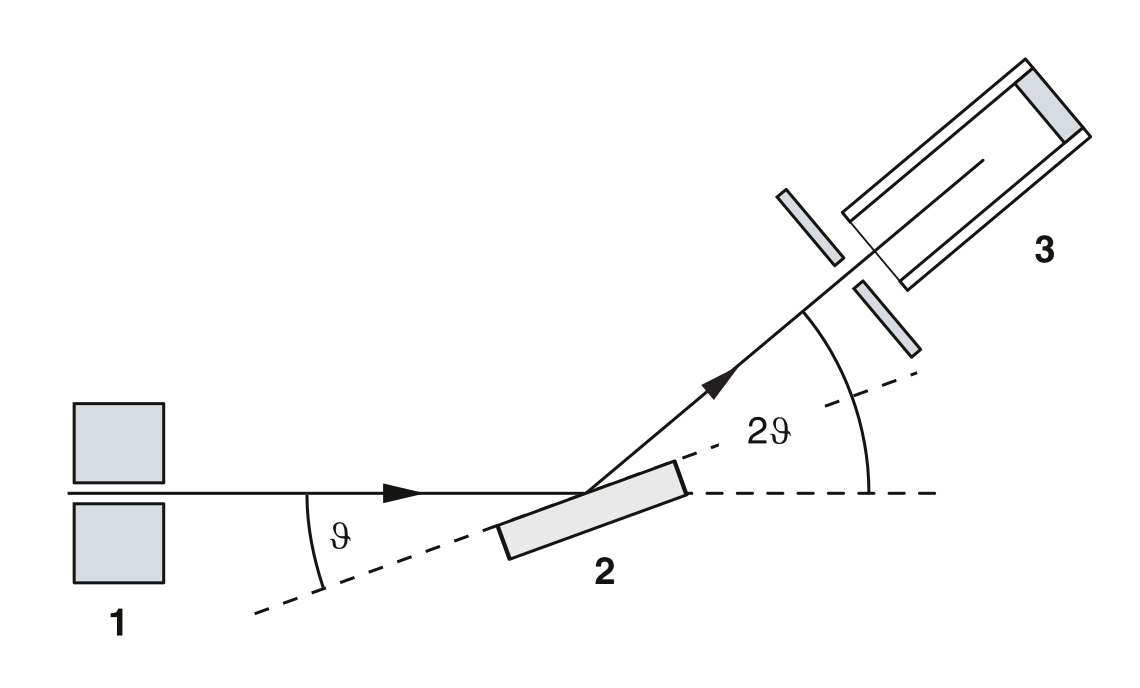
\includegraphics[width=0.4\textwidth]{media/setup.png}
  \caption{Diagram showing the principle of diffraction of x-rays at a
monocrystal and 2q coupling between counter-tube angle
and scattering angle (glancing angle)
1 collimator, 2 monocrystal, 3 counter tube. Taken from the laboratory manual.}
  \label{fig:setup}
\end{figure}

\subsection{X-Ray Source}
\label{sec:X-Ray Source}
For this lab a x-ray source with a molybdenum anode is used. It has two characteristic wave lengths 
\begin{align*}
  \lambda (K_\alpha) &= \SI{71.08}{pm} \\
  \lambda (K_\beta) &= \SI{63.09}{pm}
\end{align*}
which are given in the manual. These values will be tested in the first part of the experiment using
the known lattice constant of NaCl.

\subsection{Sample and Detector}
\label{sec:Sample and Detector}
As a x-ray detector a Geiger tube is used. It and the sample are attached to servo motors which can
rotate both independently. In this experiment however, the sample is tilted by the angle $\theta$
and the detector by $2\theta$ perpendicular to the original x-ray beam path to look for reflections
according to the basic laws of reflections.

A computer is controlling the motors and counts the events detected at the Geiger detector. As a
setting we will use
\begin{align*}
  \Delta \theta &= 0.1^\circ \\
  \Delta t &= \SI{10}{s}
\end{align*}
as a good balance between runtime and accuracy.

